\section{Error handling}
\label{sec:impl:errorhandling}
\begin{figure}[!h]
  \centering
    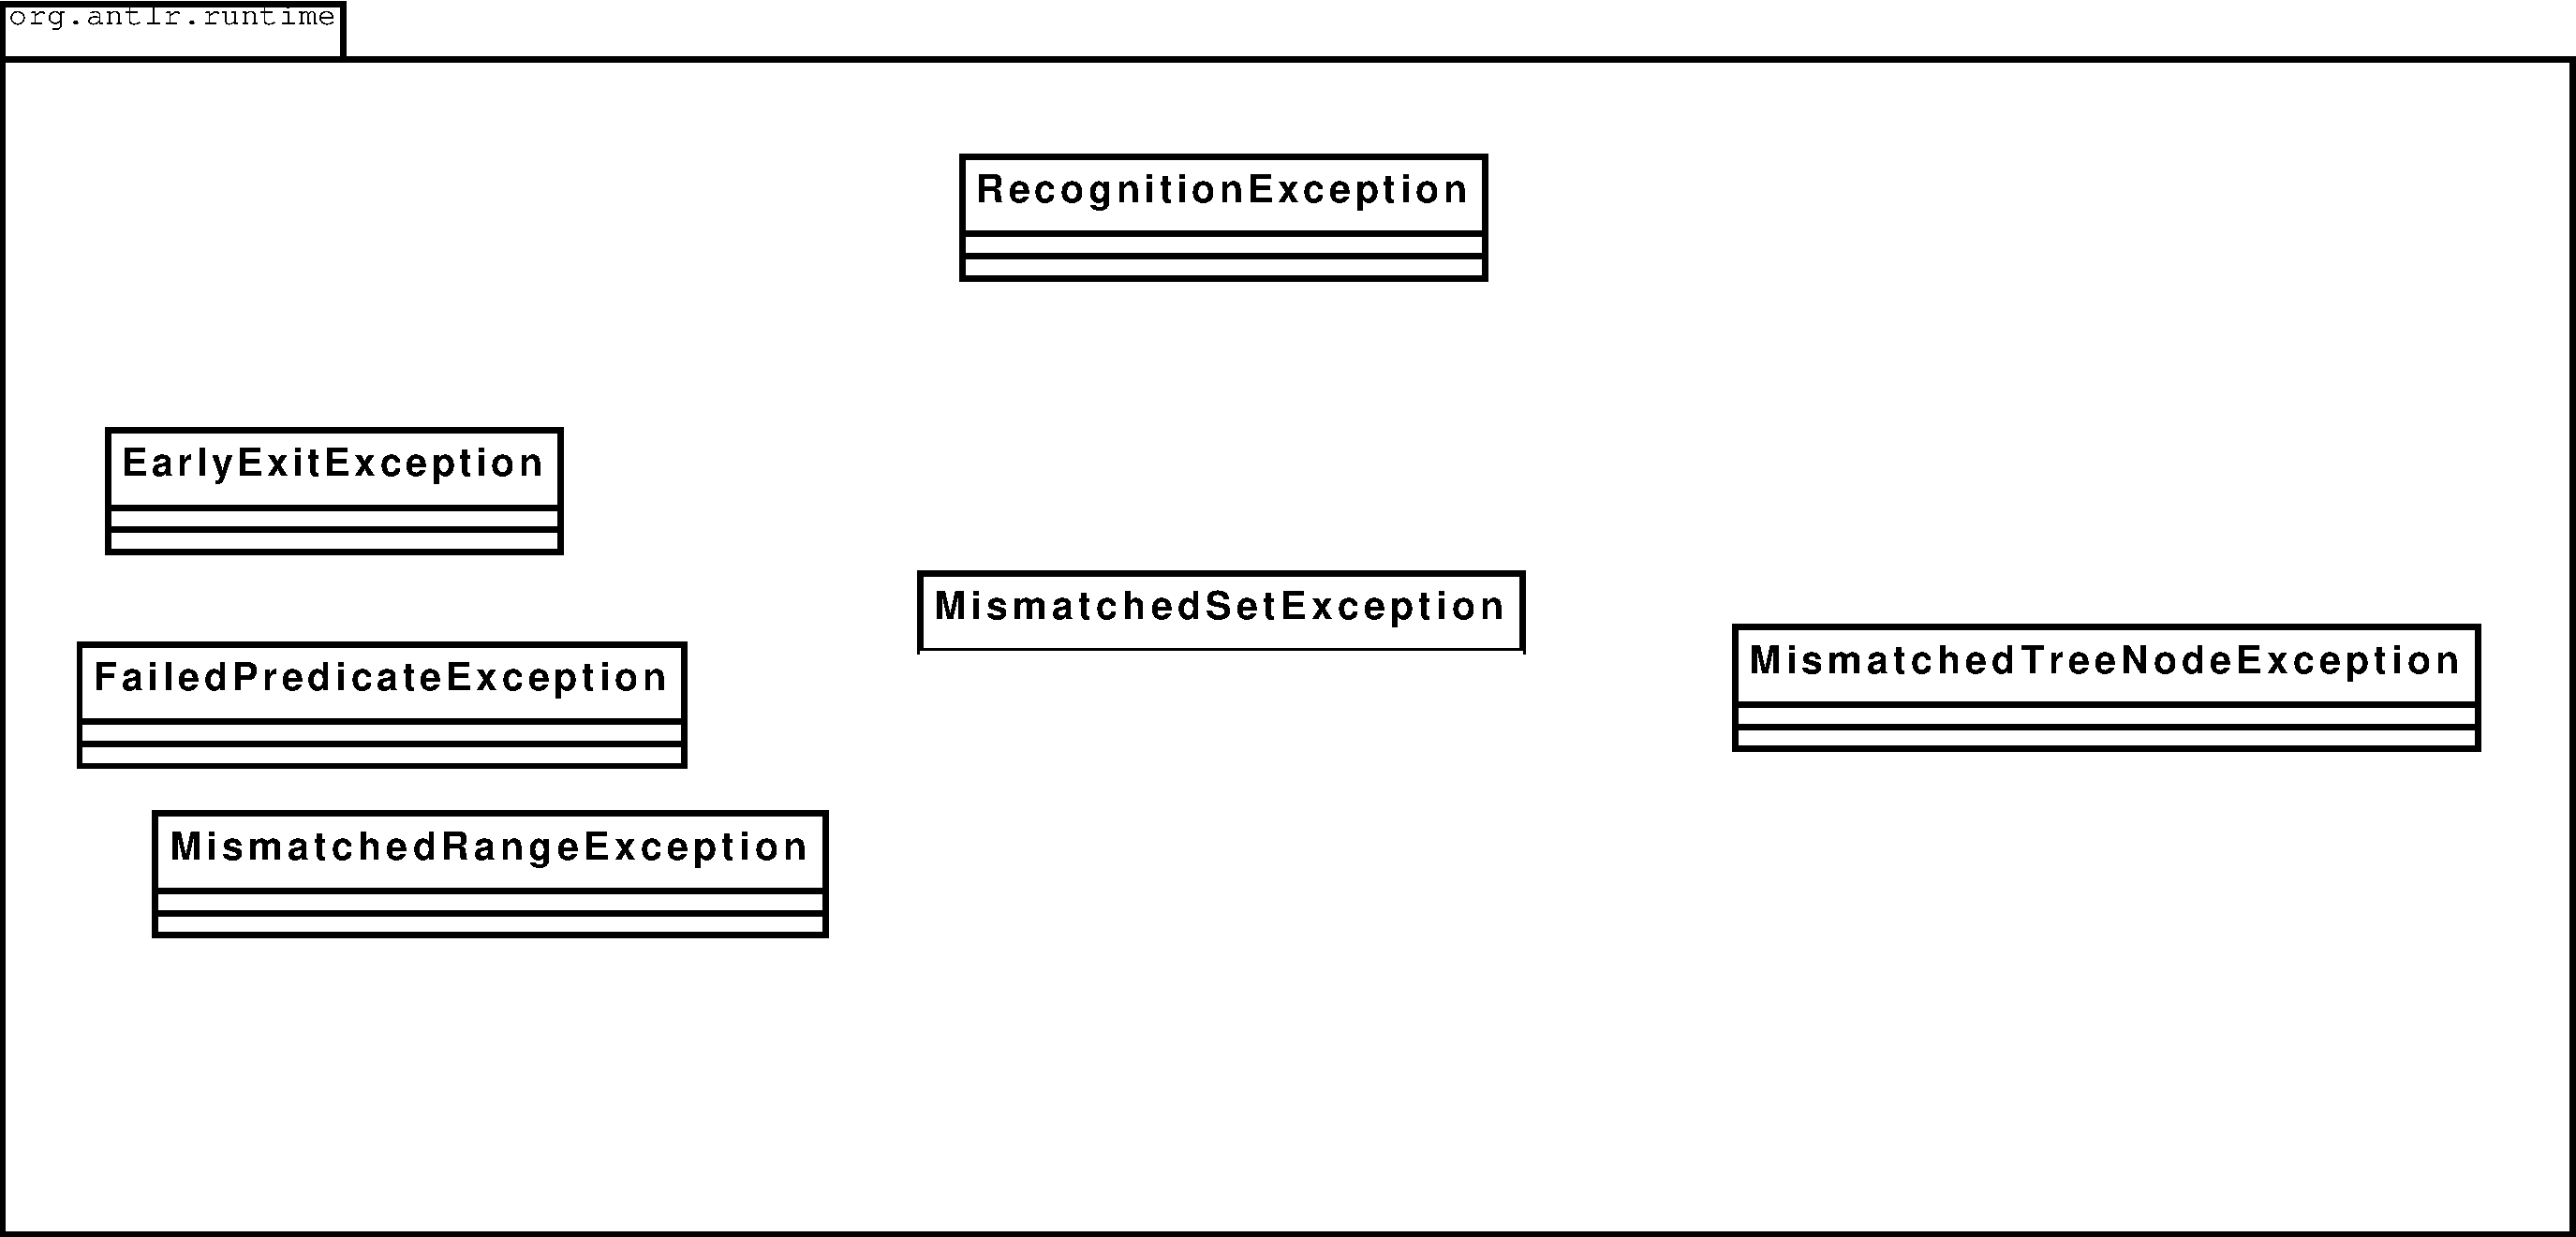
\includegraphics[width=1\textwidth]{img/exception_uml.png}
  \caption{ANTLR exceptions class hierarchy}
\end{figure}
Error handling in ANTLR is initially done by catching exceptions and printing
an error message to stderr. The parser will then attempt to recover from the
error and continue parsing. This behaviour is not always desirable, so certain
methods were overridden to allow exceptions to be thrown up the stack to the
program that initiated the parser.

Specifically, this was done by overriding the methods mismatch() as well as
recoverFromMismatchedSet(), as such:

\begin{verbatim}
    protected void mismatch(IntStream input, 
                            int ttype, 
                            BitSet follow)
        throws RecognitionException
    {
        throw new MismatchedTokenException(ttype, input);
    }

    public void recoverFromMismatchedSet(IntStream input, 
                                         RecognitionException e, 
                                         BitSet follow)
        throws RecognitionException
    {
        throw e;
    }
\end{verbatim}

Additionally, a special @rulecatch rule had to be added to force ANTLR from
handling errors and instead throwing the exceptions upwards:

\begin{verbatim}
@rulecatch {
    catch (RecognitionException e) {
        throw e;
    }
}
\end{verbatim}